% !TeX program = xelatex
% ============================================================
% 2000 年·广东卷（科类未标） · 解析版
% 由 tools/make_editions.py 生成（重跑会覆盖本文件）；
% 题目/解析内容在 questions.tex / answers*.tex，勿在本文件内写内容。
% ============================================================
\documentclass[zihao=-4, a4paper]{ctexart}
% ============================================================
% common/preamble.tex —— 拆分版试卷项目 · 公共导言区
% 引擎：XeLaTeX；文档类 ctexart 由各版本壳文件自行声明
% 由合并书 math-gaokao-2017-2026/preamble.tex 改造而来：
%   - 页眉左右改为可重定义宏 \gkheadL / \gkheadR（各版本壳设置）
%   - hyperref 不再写死 pdftitle（壳内 \hypersetup 覆盖）
%   - 删除书籍专用的 \chaptermark 重定义与 \gkpaper 装配宏
% ============================================================

% ---------- 数学 ----------
\usepackage{amsmath}
\usepackage{amssymb}
\usepackage{mathtools}

% ---------- 绘图 ----------
\usepackage{tikz}
\usetikzlibrary{shapes.geometric, arrows.meta, calc, patterns, angles, quotes, positioning}
\usepackage{pgfplots}
\pgfplotsset{compat=1.18}

% ---------- 版面 ----------
\usepackage{geometry}
\usepackage{needspace}
\geometry{a4paper, margin=2.2cm, headheight=15pt}
% 紧凑版式（如印刷版）可在壳文件中于 \begin{document} 前再次调用 \geometry 覆盖
\usepackage{enumitem}
\setlist{itemsep=2pt, topsep=4pt, parsep=0pt}

% 中文与行内公式混排的断行弹性：
% emergencystretch 允许段落末路不通时追加伸展量；
% 降低二元/关系符罚分，允许行内长公式在 = 、+ 等处断行（否则整段外溢）
\emergencystretch=2em
\binoppenalty=700
\relpenalty=500
\usepackage{booktabs}      % 三线表
\usepackage[most]{tcolorbox}

% ---------- 选择题选项对齐 ----------
% tasks 宏包：\begin{gkopts}(列数) \task ... \end{gkopts}
% 自动等宽分栏，选项天然对齐；列数已由内容片段按选项长度写定（4/2/1）
\usepackage{tasks}
\settasks{label={}, label-width=0pt, item-indent=1.2em,
          column-sep=1em, after-item-skip=2pt, before-skip=2pt, after-skip=4pt}
\NewTasksEnvironment[style=itemize]{gkopts}[\task](4)

% ---------- 页眉页脚 ----------
\newcommand{\gkheadL}{}   % 左页眉：卷名（壳文件 \renewcommand 设置）
\newcommand{\gkheadR}{}   % 右页眉：版本名（壳文件 \renewcommand 设置）
\usepackage{fancyhdr}
\pagestyle{fancy}
\fancyhf{}
\fancyhead[L]{\small\gkheadL}
\fancyhead[R]{\small\gkheadR}
\fancyfoot[C]{\small —— 第 \thepage\ 页 ——}
\renewcommand{\headrulewidth}{0.4pt}

% ---------- 超链接（须最后加载）----------
\usepackage{hyperref}
\hypersetup{colorlinks=true, linkcolor=blue!55!black,
            bookmarksnumbered=true, unicode=true}

% ============================================================
% common/macros.tex —— 自定义命令与环境（题号、解析头、提示框等）
% 与合并书 math-gaokao-2017-2026/preamble.tex 的自定义段保持一致，
% 保证内容片段（questions.tex / answers.tex）在两个项目间可互换。
% ============================================================

% ---------- 试卷标识（壳文件 \renewcommand 设置，用于 label 命名空间）----------
\newcommand{\gkpaperid}{none}

% ---------- 题号 ----------
% 试题部分的题号：加粗编号 + 自动 \label{q:<卷id>:<题号>}
\newcommand{\gkti}[1]{\par\medskip\noindent
  \textbf{#1．}\phantomsection\label{q:\gkpaperid:#1}\ignorespaces}
% 多卷/分部重启题号时，#1 是唯一内部顺序号（交叉引用身份），#2 才是原卷显示题号。
\newcommand{\gktiwithlabel}[2]{\par\medskip\noindent
  \textbf{#2．}\phantomsection\label{q:\gkpaperid:#1}\ignorespaces}

% 解析部分的题头：小标题 + 回链到试题页
% （仅在题目与解析同文档的版本中回链有效；试题版不含解析头，无悬空引用）
\newcommand{\gksolhead}[2]{%
  \Needspace{3\baselineskip}\subsubsection*{第 #1 题\if\relax\detokenize{#2}\relax\else（#2）\fi}%
  \phantomsection\label{s:\gkpaperid:#1}%
  {\small\color{gray}（题目见第~\pageref{q:\gkpaperid:#1}~页）}\par\nopagebreak}
% 与 \gktiwithlabel 成对：显示原题号，但回链仍用唯一内部顺序号。
\newcommand{\gksolheadwithlabel}[3]{%
  \Needspace{3\baselineskip}\subsubsection*{第 #2 题\if\relax\detokenize{#3}\relax\else（#3）\fi}%
  \phantomsection\label{s:\gkpaperid:#1}%
  {\small\color{gray}（题目见第~\pageref{q:\gkpaperid:#1}~页）}\par\nopagebreak}

% ---------- 填空题空位 ----------
\newcommand{\gkblank}{\underline{\hspace{2.2em}}}

% ---------- 提示框 ----------
% 卷种提示 / 解析归属声明（醒目，浅黄）
\newtcolorbox{gknotice}{colback=yellow!8, colframe=orange!60!black,
  boxrule=0.5pt, arc=1.5pt, left=6pt, right=6pt, top=4pt, bottom=4pt,
  before skip=8pt, after skip=8pt}

% 方法提示 / 注（浅蓝，用于解析后的点评与题量说明）
\newtcolorbox{gktip}{colback=blue!4, colframe=blue!35!black,
  boxrule=0.4pt, arc=1.5pt, left=6pt, right=6pt, top=4pt, bottom=4pt,
  before skip=6pt, after skip=6pt, fontupper=\small}

% ---------- 答案行 ----------
% 解析中独立成段的"答案：X"用带底色的行呈现
\newcommand{\gkanswer}[1]{\par\smallskip\noindent
  \tcbox[width=\linewidth, tcbox width=auto limited,
         colback=green!6, colframe=green!35!black, boxrule=0.4pt,
         arc=1.5pt, left=4pt, right=4pt, top=2pt, bottom=2pt,
         nobeforeafter]{\textbf{#1}}\par\smallskip}

% ---------- 结构标题 ----------
% 结构标题后通常紧跟一个带 0.5\textheight 起始预留的解析题块；0.4 只够放标题，
% 会把下一题整体推到下一页，留下孤立的「二、填空题」等页尾标题。
\newcommand{\gkpart}[1]{\Needspace{0.6\textheight}\subsection*{#1}\nopagebreak}     % 标题 + 首题
% （一）必考题 / 解析小问标题：块式加粗段，可自动换行（\paragraph 的 run-in 版式会溢出）
\newcommand{\gksubpart}[1]{\Needspace{6\baselineskip}\par\medskip\noindent\textbf{#1}\par\nopagebreak\smallskip}

% 罗马数字Ⅰ-Ⅻ（U+2160）与圈号①②③（U+2460）划入 CJK 字符类，
% 用中文字体渲染——西文字体 Latin Modern 缺这些字形，否则整段静默丢字
\xeCJKDeclareCharClass{CJK}{"2160 -> "217F, "2460 -> "24FF}

% ============================================================
% common/questions_env.tex —— 题目 / 解析的语义包装环境
%
% questions.tex 中每道题包在 \begin{question}...\end{question} 里，
% answers.tex 中每题解析包在 \begin{answer}...\end{answer} 里；
% 题头排版仍由内容行中的 \gkti / \gksolhead 完成（见 macros.tex）。
%
% 环境本身不产生任何盒子或垂直间距（只引入一个 TeX 分组），
% 排版结果与不包裹时逐点一致。它的价值在于：
%   1. 给每道题一个机器可数的结构边界（校验脚本数环境数 = 题量）；
%   2. 为将来的条件编译留钩子——某版本可重定义环境实现按题取舍。
% ============================================================

% 环境不把整题装盒：题目与解析仍可自然跨页，但开始题块前必须为题面、
% 图形/表格或解析首段留出足够空间。仅保留 2 个 baseline 会让题干、
% 选项和图形在页边界处被拆开，形成不可打印的孤立内容；题目保留
% 0.15\textheight，在避免短题制造大段空白与避免题块拆分之间取平衡。
% 解析题块保留 0.5\textheight，以容纳“题面 + 图形/选项 + 首段解析”；
% 结构标题仍用更大的保留量；末页自然收尾由视觉复审判定。
\newenvironment{question}{\Needspace{0.15\textheight}}{}
\newenvironment{answer}{\Needspace{0.5\textheight}}{}

\renewcommand{\gkpaperid}{gk-2000-regular-guangdong-unspecified}
\renewcommand{\gkheadL}{2000 年·广东卷（科类未标） · 数学}
\renewcommand{\gkheadR}{解析版}
\hypersetup{pdftitle={2000 年·广东卷（科类未标） 数学 · 解析版}}
\begin{document}
\begin{center}
  {\Large\bfseries 2000 年·广东卷（科类未标）}\\[4pt]
  {\large 数学 · 解析版}
\end{center}
\medskip
\pdfbookmark[1]{试题}{sec:q}
% questions.tex —— 2000 年·广东卷（科类未标） · 题目内容片段（无答案）
% 由 tools/generate_projects.py 依来源总账自 2000/2000_数学真题_广东_试题.md 生成，勿手改（改源 MD 后重跑）


\begin{gktip}
\textbf{来源说明}：固定副本题签自题“2000 普通高等学校招生考试（广东卷）”。固定源只含题面，不含答案或解析；科类、发布者、出版物和版本身份未核。答案与解析为本库独立推导，不能称为官方标准答案。

\textbf{图稿说明}：Q5、Q12、Q16、Q19、Q21、Q22保留固定扫描中的图形关系；项目图稿已创建，仍待正式构建目视核对。
\end{gktip}

\gkpart{一、选择题}

\begin{question}
\gkti{1}已知集合 $A=\{1,2,3,4\}$，那么 $A$ 的真子集的个数是\mbox{（　　）}。

（A）15　　（B）16　　（C）3　　（D）4

\end{question}
\begin{question}
\gkti{2}在复平面内，把复数 $3-\sqrt{3}i$ 对应的向量按顺时针方向旋转 $\dfrac{\pi}{3}$，所得向量对应的复数是\mbox{（　　）}。

（A）$2\sqrt{3}$　　（B）$-2\sqrt{3}i$　　（C）$\sqrt{3}-3i$　　（D）$3+\sqrt{3}i$

\end{question}
\begin{question}
\gkti{3}一个长方体共一顶点的三个面的面积分别是 $\sqrt{2},\sqrt{3},\sqrt{6}$，这个长方体对角线的长是\mbox{（　　）}。

（A）$2\sqrt{3}$　　（B）$3\sqrt{2}$　　（C）$6$　　（D）$\sqrt{6}$

\end{question}
\begin{question}
\gkti{4}已知 $\sin\alpha>\sin\beta$，那么下列命题成立的是\mbox{（　　）}。

（A）若 $\alpha,\beta$ 是第一象限角，则 $\cos\alpha>\cos\beta$

（B）若 $\alpha,\beta$ 是第二象限角，则 $\tan\alpha>\tan\beta$

（C）若 $\alpha,\beta$ 是第三象限角，则 $\cos\alpha>\cos\beta$

（D）若 $\alpha,\beta$ 是第四象限角，则 $\tan\alpha>\tan\beta$

\Needspace{0.4\textheight}
\end{question}
\begin{question}
\gkti{5}函数 $y=-x\cos x$ 的部分图象是\mbox{（　　）}。
\nopagebreak[4]
\begin{center}% 2000 年广东卷第 5 题：函数 -x cos x 的四个图象选项
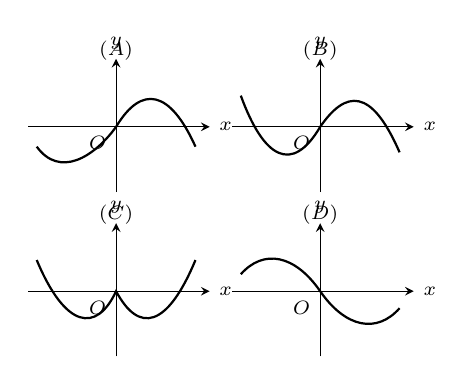
\begin{tikzpicture}[>=stealth, scale=0.72]
  \begin{scope}
    \node[font=\scriptsize] at (0,1.35) {$(A)$};
    \draw[->] (-1.55,0)--(1.65,0) node[right, font=\scriptsize] {$x$};
    \draw[->] (0,-1.15)--(0,1.2) node[above, font=\scriptsize] {$y$};
    \draw[thick] (-1.4,-0.35) .. controls (-1.0,-0.9) and (-0.4,-0.55) .. (0,0)
      .. controls (0.45,0.75) and (0.95,0.65) .. (1.4,-0.35);
    \node[below left, font=\scriptsize] at (0,0) {$O$};
  \end{scope}

  \begin{scope}[xshift=3.6cm]
    \node[font=\scriptsize] at (0,1.35) {$(B)$};
    \draw[->] (-1.55,0)--(1.65,0) node[right, font=\scriptsize] {$x$};
    \draw[->] (0,-1.15)--(0,1.2) node[above, font=\scriptsize] {$y$};
    \draw[thick] (-1.4,0.55) .. controls (-1.0,-0.55) and (-0.5,-0.85) .. (0,0)
      .. controls (0.45,0.65) and (0.9,0.7) .. (1.4,-0.45);
    \node[below left, font=\scriptsize] at (0,0) {$O$};
  \end{scope}

  \begin{scope}[yshift=-2.9cm]
    \node[font=\scriptsize] at (0,1.35) {$(C)$};
    \draw[->] (-1.55,0)--(1.65,0) node[right, font=\scriptsize] {$x$};
    \draw[->] (0,-1.15)--(0,1.2) node[above, font=\scriptsize] {$y$};
    \draw[thick] (-1.4,0.55) .. controls (-0.9,-0.65) and (-0.35,-0.75) .. (0,0)
      .. controls (0.4,-0.75) and (0.9,-0.65) .. (1.4,0.55);
    \node[below left, font=\scriptsize] at (0,0) {$O$};
  \end{scope}

  \begin{scope}[xshift=3.6cm,yshift=-2.9cm]
    \node[font=\scriptsize] at (0,1.35) {$(D)$};
    \draw[->] (-1.55,0)--(1.65,0) node[right, font=\scriptsize] {$x$};
    \draw[->] (0,-1.15)--(0,1.2) node[above, font=\scriptsize] {$y$};
    \draw[thick] (-1.4,0.3) .. controls (-1.0,0.75) and (-0.45,0.65) .. (0,0)
      .. controls (0.45,-0.65) and (1.0,-0.75) .. (1.4,-0.3);
    \node[below left, font=\scriptsize] at (0,0) {$O$};
  \end{scope}
\end{tikzpicture}
\end{center}
\nopagebreak[4]
\end{question}
\begin{question}
\gkti{6}《中华人民共和国个人所得税法》规定，公民全月工资、薪金所得不超过 800 元的部分不必纳税，超过 800 元的部分为全月应纳税所得额，此项税款按下表分段累进计算：

\begin{center}
\begin{tabular}{lr}
\toprule
全月应纳税所得额 & 税率 \\
\midrule
不超过 500 元的部分 & 5\% \\
超过 500 元至 2000 元的部分 & 10\% \\
超过 2000 元至 5000 元的部分 & 15\% \\
…… & …… \\
\bottomrule
\end{tabular}
\end{center}

某人一月份交纳此项税款 26.78 元，则他的当月工资、薪金所得介于\mbox{（　　）}。

（A）800–900 元　　（B）900–1200 元　　（C）1200–1500 元　　（D）1500–2800 元

\end{question}
\begin{question}
\gkti{7}若 $a>b>1$，$P=\sqrt{\lg a\cdot\lg b}$，$Q=\dfrac{1}{2}(\lg a+\lg b)$，$R=\lg\left(\dfrac{a+b}{2}\right)$，则\mbox{（　　）}。

（A）$R<P<Q$　　（B）$P<Q<R$　　（C）$Q<P<R$　　（D）$P<R<Q$

\end{question}
\begin{question}
\gkti{8}以极坐标系中的点 $(1,1)$ 为圆心、1 为半径的圆的方程是\mbox{（　　）}。

（A）$\rho=2\cos\left(\theta-\dfrac{\pi}{4}\right)$　　（B）$\rho=2\sin\left(\theta-\dfrac{\pi}{4}\right)$

（C）$\rho=2\cos(\theta-1)$　　（D）$\rho=2\sin(\theta-1)$

\end{question}
\begin{question}
\gkti{9}一个圆柱的侧面展开图是一个正方形，这个圆柱的全面积与侧面积的比是\mbox{（　　）}。

（A）$\dfrac{1+2\pi}{2\pi}$　　（B）$\dfrac{1+4\pi}{4\pi}$　　（C）$\dfrac{1+2\pi}{\pi}$　　（D）$\dfrac{1+4\pi}{2\pi}$

\end{question}
\begin{question}
\gkti{10}过原点的直线与圆 $x^2+y^2+4x+3=0$ 相切，若切点在第三象限，则该直线的方程是\mbox{（　　）}。

（A）$y=\sqrt{3}x$　　（B）$y=-\sqrt{3}x$　　（C）$y=\dfrac{\sqrt{3}}{3}x$　　（D）$y=-\dfrac{\sqrt{3}}{3}x$

\end{question}
\begin{question}
\gkti{11}过抛物线 $y=ax^2\ (a>0)$ 的焦点 $F$ 作一直线交抛物线于 $P,Q$ 两点，若线段 $PF$ 与 $FQ$ 的长分别是 $p,q$，则 $\dfrac{1}{p}+\dfrac{1}{q}$ 等于\mbox{（　　）}。

（A）$2a$　　（B）$\dfrac{1}{2a}$　　（C）$4a$　　（D）$\dfrac{4}{a}$

\Needspace{0.4\textheight}
\end{question}
\begin{question}
\gkti{12}如图，$OA$ 是圆锥底面中心 $O$ 到母线的垂线，$OA$ 绕轴旋转一周所得曲面将圆锥分成体积相等的两部分，则母线与轴的夹角的余弦值为\mbox{（　　）}。
\nopagebreak[4]
\begin{center}% 2000 年广东卷第 12 题：圆锥轴截面与 OA
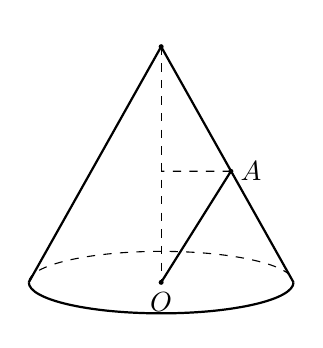
\begin{tikzpicture}[>=stealth, scale=0.82]
  \coordinate (V) at (0,3.65);
  \coordinate (O) at (0,0);
  \coordinate (L) at (-2.05,0);
  \coordinate (R) at (2.05,0);
  \coordinate (A) at (1.08,1.72);
  \draw[thick] (V)--(L) (V)--(R);
  \draw[thick] (L) arc (180:360:2.05 and 0.48);
  \draw[dashed] (L) arc (180:0:2.05 and 0.48);
  \draw[dashed] (V)--(O);
  \draw[thick] (O)--(A);
  \draw[dashed] (A)--(0,1.72);
  \fill (V) circle (1.1pt);
  \fill (O) circle (1.1pt) node[below] {$O$};
  \fill (A) circle (1.1pt) node[right] {$A$};
  \node[above] at (V) { };
\end{tikzpicture}
\end{center}
\nopagebreak[4]
（A）$\dfrac{1}{\sqrt[3]{2}}$　　（B）$\dfrac{1}{2}$　　（C）$\dfrac{1}{\sqrt{2}}$　　（D）$\dfrac{1}{\sqrt[4]{2}}$

\end{question}
\gkpart{二、填空题}

\begin{question}
\gkti{13}乒乓球队的 10 名队员中有 3 名主力队员，派 5 名参加比赛，3 名主力队员要安排在第一、三、五位置，其余 7 名队员选 2 名安排在第二、四位置，那么不同的出场安排共有 \gkblank{} 种（用数字作答）。

\end{question}
\begin{question}
\gkti{14}椭圆 $\dfrac{x^2}{9}+\dfrac{y^2}{4}=1$ 的焦点为 $F_1,F_2$，$P$ 为其上的动点，当 $\angle F_1PF_2$ 为钝角时，点 $P$ 横坐标的取值范围是 \gkblank{}。

\end{question}
\begin{question}
\gkti{15}设 $\{a_n\}$ 是首项为 1 的正项数列，且
\nopagebreak[4]
\[
(n+1)a_{n+1}^{2}-na_n^{2}+a_{n+1}a_n=0\qquad(n=1,2,3,\ldots),
\]
则它的通项公式是 $a_n=$ \gkblank{}。

\Needspace{0.4\textheight}
\end{question}
\begin{question}
\gkti{16}如图，$E,F$ 分别为正方体面 $ADD_1A_1$、面 $BCC_1B_1$ 的中心，则四边形 $BFD_1E$ 在该正方体的面上的射影可能是 \gkblank{}。（要求：把可能的图序号都填上。）
\nopagebreak[4]
\begin{center}% 2000 年广东卷第 16 题：正方体内四边形投影的可能图形
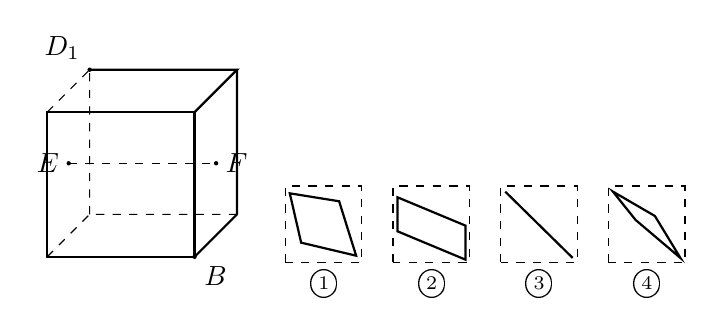
\begin{tikzpicture}[>=stealth, scale=0.72]
  \coordinate (A) at (0,0);
  \coordinate (B) at (2.6,0);
  \coordinate (C) at (3.35,0.75);
  \coordinate (D) at (0.75,0.75);
  \coordinate (A1) at (0,2.55);
  \coordinate (B1) at (2.6,2.55);
  \coordinate (C1) at (3.35,3.3);
  \coordinate (D1) at (0.75,3.3);
  \coordinate (E) at (0.38,1.65);
  \coordinate (F) at (2.98,1.65);

  \draw[thick] (A)--(B)--(B1)--(A1)--cycle;
  \draw[thick] (B1)--(C1)--(D1);
  \draw[dashed] (A)--(D)--(C) (D)--(D1) (A1)--(D1);
  \draw[thick] (B)--(C) (C)--(C1);
  \draw[dashed] (E)--(F);
  \fill (B) circle (1.1pt) node[below right] {$B$};
  \fill (D1) circle (1.1pt) node[above left] {$D_1$};
  \fill (E) circle (1.1pt) node[left] {$E$};
  \fill (F) circle (1.1pt) node[right] {$F$};

  \begin{scope}[xshift=4.2cm,yshift=-0.1cm]
    \draw[dashed] (0,0) rectangle (1.35,1.35);
    \draw[thick] (0.08,1.22)--(0.95,1.08)--(1.25,0.12)--(0.28,0.35)--cycle;
    \node[below] at (0.68,-0.08) {\textcircled{\scriptsize 1}};
  \end{scope}
  \begin{scope}[xshift=6.1cm,yshift=-0.1cm]
    \draw[dashed] (0,0) rectangle (1.35,1.35);
    \draw[thick] (0.08,1.15)--(0.08,0.55)--(1.28,0.05)--(1.28,0.65)--cycle;
    \node[below] at (0.68,-0.08) {\textcircled{\scriptsize 2}};
  \end{scope}
  \begin{scope}[xshift=8.0cm,yshift=-0.1cm]
    \draw[dashed] (0,0) rectangle (1.35,1.35);
    \draw[thick] (0.08,1.25)--(1.27,0.08);
    \node[below] at (0.68,-0.08) {\textcircled{\scriptsize 3}};
  \end{scope}
  \begin{scope}[xshift=9.9cm,yshift=-0.1cm]
    \draw[dashed] (0,0) rectangle (1.35,1.35);
    \draw[thick] (0.08,1.25)--(0.48,0.75)--(1.27,0.08)--(0.82,0.82)--cycle;
    \node[below] at (0.68,-0.08) {\textcircled{\scriptsize 4}};
  \end{scope}
\end{tikzpicture}
\end{center}
\nopagebreak[4]
\end{question}
\gkpart{三、解答题}

\begin{question}
\gkti{17}已知函数 $y=\sqrt{3}\sin x+\cos x$，$x\in\mathbb{R}$。

（1） 当函数 $y$ 取得最大值时，求自变量 $x$ 的集合；

（2） 该函数的图象可由 $y=\sin x\ (x\in\mathbb{R})$ 的图象经过怎样的平移和伸缩变换得到？

\end{question}
\begin{question}
\gkti{18}设 $\{a_n\}$ 为等比数列，
\nopagebreak[4]
\[
T_n=na_1+(n-1)a_2+\cdots+2a_{n-1}+a_n,
\]
已知 $T_1=1,\ T_2=4$。

（1） 求数列 $\{a_n\}$ 的首项和公比；

（2） 求数列 $\{T_n\}$ 的通项公式。

\Needspace{0.4\textheight}
\end{question}
\begin{question}
\gkti{19}如图，已知平行六面体 $ABCD-A_1B_1C_1D_1$ 的底面 $ABCD$ 上菱形，且 $\angle C_1CB=\angle C_1CD=\angle BCD$。

\begin{gktip}
\textbf{源文待核（ISSUE-1201）}：固定扫描件照录为“底面 $ABCD$ 上菱形”；此处语义不通，暂不擅自补字或改写。
\end{gktip}

（1） 证明：$C_1C\perp BD$；

（2） 当 $\dfrac{CD}{CC_1}$ 的值为多少时，能使 $A_1C\perp$ 平面 $C_1BD$？请给出证明。
\nopagebreak[4]
\begin{center}% 2000 年广东卷第 19 题：平行六面体 ABCD-A1B1C1D1
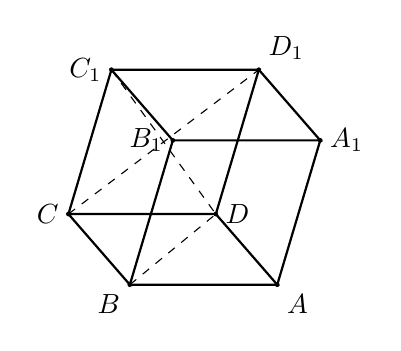
\begin{tikzpicture}[>=stealth, scale=0.78]
  \coordinate (A) at (3.4,0);
  \coordinate (B) at (1.0,0);
  \coordinate (C) at (0,1.15);
  \coordinate (D) at (2.4,1.15);
  \coordinate (A1) at (4.1,2.35);
  \coordinate (B1) at (1.7,2.35);
  \coordinate (C1) at (0.7,3.5);
  \coordinate (D1) at (3.1,3.5);

  \draw[thick] (A)--(B)--(C)--(D)--cycle;
  \draw[thick] (A1)--(B1)--(C1)--(D1)--cycle;
  \draw[thick] (A)--(A1) (B)--(B1) (C)--(C1) (D)--(D1);
  \draw[dashed] (C1)--(D) (B)--(D) (C)--(D1);

  \fill (A) circle (1.1pt) node[below right] {$A$};
  \fill (B) circle (1.1pt) node[below left] {$B$};
  \fill (C) circle (1.1pt) node[left] {$C$};
  \fill (D) circle (1.1pt) node[right] {$D$};
  \fill (A1) circle (1.1pt) node[right] {$A_1$};
  \fill (B1) circle (1.1pt) node[left] {$B_1$};
  \fill (C1) circle (1.1pt) node[left] {$C_1$};
  \fill (D1) circle (1.1pt) node[above right] {$D_1$};
\end{tikzpicture}
\end{center}
\nopagebreak[4]
\end{question}
\begin{question}
\gkti{20}设函数 $f(x)=\sqrt{x^2+1}-ax$，其中 $a>0$。

（1） 解不等式 $f(x)\leq 1$；

（2） 证明：当 $a\geq1$ 时，函数 $f(x)$ 在区间 $[0,+\infty)$ 上是单调函数。

\Needspace{0.4\textheight}
\end{question}
\begin{question}
\gkti{21}某蔬菜基地种植西红柿，由历年市场行情得知，从二月一日起的 300 天内，西红柿市场售价与上市时间的关系用图一的一条折线表示；西红柿的种植成本与上市时间的关系用图二的抛物线段表示。

（1） 写出图一表示的市场售价与时间的函数关系式 $p=f(t)$ 和图二表示的种植成本与时间的函数关系式 $Q=g(t)$；

（2） 认定市场售价减去种植成本为纯收益，问何时上市的西红柿纯收益最大？

注：市场售价各种植成本的单位：元/$10^2\,\mathrm{kg}$，时间单位：天。
\nopagebreak[4]
\begin{center}% 2000 年广东卷第 21 题：市场售价与种植成本图象
\begin{tikzpicture}[>=stealth, scale=0.78]
  \begin{scope}
    \draw[->] (0,0)--(3.55,0) node[right] {$t$};
    \draw[->] (0,0)--(0,3.65) node[above] {$P$};
    \draw[thick] (0,3.0)--(2.0,1.0)--(3.0,3.0);
    \draw[dashed] (0,3.0)--(3.0,3.0) (0,1.0)--(2.0,1.0)
      (2.0,0)--(2.0,1.0) (3.0,0)--(3.0,3.0);
    \node[left, font=\scriptsize] at (0,3.0) {300};
    \node[left, font=\scriptsize] at (0,1.0) {100};
    \node[below, font=\scriptsize] at (2.0,0) {200};
    \node[below, font=\scriptsize] at (3.0,0) {300};
    \node[below] at (1.5,-0.42) {图一};
  \end{scope}
  \begin{scope}[xshift=4.35cm]
    \draw[->] (0,0)--(3.55,0) node[right] {$t$};
    \draw[->] (0,0)--(0,3.65) node[above] {$Q$};
    \draw[thick, domain=0:3, samples=80]
      plot (\x,{1+(\x-1.5)^2/2});
    \draw[dashed] (0,1)--(3,1) (0,1.5)--(0.5,1.5) (0,1.5)--(2.5,1.5)
      (0.5,0)--(0.5,1.5) (1.5,0)--(1.5,1) (2.5,0)--(2.5,1.5);
    \node[left, font=\scriptsize] at (0,3.0) {300};
    \node[left, font=\scriptsize] at (0,2.5) {250};
    \node[left, font=\scriptsize] at (0,1.5) {150};
    \node[left, font=\scriptsize] at (0,1.0) {100};
    \node[below, font=\scriptsize] at (0.5,0) {50};
    \node[below, font=\scriptsize] at (1.5,0) {150};
    \node[below, font=\scriptsize] at (2.5,0) {250};
    \node[below] at (1.5,-0.42) {图二};
  \end{scope}
\end{tikzpicture}
\end{center}
\nopagebreak[4]
\Needspace{0.4\textheight}
\end{question}
\begin{question}
\gkti{22}如图，已知梯形 $ABCD$ 中 $|AB|=2|CD|$，点 $E$ 分有向线段 $AC$ 所成的比为 $\lambda$，双曲线过 $C,D,E$ 三点，且以 $A,B$ 为焦点。当 $\dfrac{2}{3}\leq\lambda\leq\dfrac{3}{4}$ 时，求双曲线离心率 $e$ 的取值范围。
\nopagebreak[4]
\begin{center}% 2000 年广东卷第 22 题：梯形、分点与双曲线
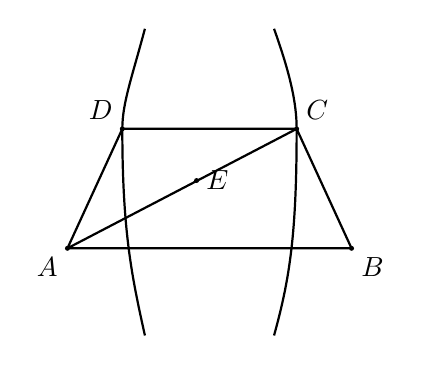
\begin{tikzpicture}[>=stealth, scale=0.82]
  \coordinate (A) at (0,0);
  \coordinate (B) at (4.4,0);
  \coordinate (D) at (0.85,1.85);
  \coordinate (C) at (3.55,1.85);
  \coordinate (E) at (2.0,1.05);

  \draw[thick] (A)--(B)--(C)--(D)--cycle;
  \draw[thick] (A)--(C);
  \draw[thick] (1.2,3.4) .. controls (1.0,2.65) and (0.85,2.25) .. (0.85,1.85);
  \draw[thick] (3.2,3.4) .. controls (3.45,2.7) and (3.55,2.25) .. (3.55,1.85);
  \draw[thick] (1.2,-1.35) .. controls (1.0,-0.45) and (0.85,0.25) .. (0.85,1.85);
  \draw[thick] (3.2,-1.35) .. controls (3.45,-0.45) and (3.55,0.25) .. (3.55,1.85);

  \fill (A) circle (1.1pt) node[below left] {$A$};
  \fill (B) circle (1.1pt) node[below right] {$B$};
  \fill (C) circle (1.1pt) node[above right] {$C$};
  \fill (D) circle (1.1pt) node[above left] {$D$};
  \fill (E) circle (1.1pt) node[right] {$E$};
\end{tikzpicture}
\end{center}
\nopagebreak[4]

\end{question}
\clearpage
\pdfbookmark[1]{参考答案与详细解析}{sec:s}
\Needspace{8\baselineskip}
\begin{center}{\Large\bfseries 参考答案与详细解析}\end{center}
\medskip
% answers.tex —— 2000 年·广东卷（科类未标） · 参考答案与详细解析片段
% 由 tools/generate_projects.py 依来源总账自 2000/2000_数学真题_广东_试题.md + 2000/2000_数学真题_广东_解析正文.md + 2000/2000_数学真题_广东_答案要点.md 生成，勿手改（改源 MD 后重跑）


\begin{gktip}
固定来源仅含题面。以下解析为本库独立推导，不代表官方解析。Q12与题面断言冲突；Q22的结果依赖于分点比方向，均保留待核。
\end{gktip}

\gkpart{一、选择题}

\begin{answer}
\gksolhead{1}{}

\textbf{题目}：

已知集合 $A=\{1,2,3,4\}$，那么 $A$ 的真子集的个数是\mbox{（　　）}。

（A）15　　（B）16　　（C）3　　（D）4

\Needspace{4\baselineskip}
\textbf{解析}

4 元集合共有 $2^4=16$ 个子集，去掉集合本身，真子集数为 $16-1=15$，选 A。

\gkanswer{答案：A，15}

\end{answer}
\begin{answer}
\gksolhead{2}{}

\textbf{题目}：

在复平面内，把复数 $3-\sqrt{3}i$ 对应的向量按顺时针方向旋转 $\dfrac{\pi}{3}$，所得向量对应的复数是\mbox{（　　）}。

（A）$2\sqrt{3}$　　（B）$-2\sqrt{3}i$　　（C）$\sqrt{3}-3i$　　（D）$3+\sqrt{3}i$

\Needspace{4\baselineskip}
\textbf{解析}

复数对应向量按顺时针方向旋转 $\pi/3$，对应乘以 $e^{-i\pi/3}$。原复数 $3-\sqrt3 i$ 的模为 $2\sqrt3$、辐角为 $-\pi/6$；旋转后辐角为 $-\pi/2$，所得复数为 $-2\sqrt3 i$，选 B。

\gkanswer{答案：B，$-2\sqrt3 i$}

\end{answer}
\begin{answer}
\gksolhead{3}{}

\textbf{题目}：

一个长方体共一顶点的三个面的面积分别是 $\sqrt{2},\sqrt{3},\sqrt{6}$，这个长方体对角线的长是\mbox{（　　）}。

（A）$2\sqrt{3}$　　（B）$3\sqrt{2}$　　（C）$6$　　（D）$\sqrt{6}$

\Needspace{4\baselineskip}
\textbf{解析}

设三条棱长为 $x,y,z$，则三个面面积为 $xy=\sqrt2$、$yz=\sqrt3$、$zx=\sqrt6$。因此 $x^2=2$、$y^2=1$、$z^2=3$，体对角线长为 $\sqrt{x^2+y^2+z^2}=\sqrt6$，选 D。

\gkanswer{答案：D，$\sqrt6$}

\end{answer}
\begin{answer}
\gksolhead{4}{}

\textbf{题目}：

已知 $\sin\alpha>\sin\beta$，那么下列命题成立的是\mbox{（　　）}。

（A）若 $\alpha,\beta$ 是第一象限角，则 $\cos\alpha>\cos\beta$

（B）若 $\alpha,\beta$ 是第二象限角，则 $\tan\alpha>\tan\beta$

（C）若 $\alpha,\beta$ 是第三象限角，则 $\cos\alpha>\cos\beta$

（D）若 $\alpha,\beta$ 是第四象限角，则 $\tan\alpha>\tan\beta$

\Needspace{4\baselineskip}
\textbf{解析}

由于 $\sin$、$\tan$ 均以 $2\pi$ 为周期，可将第四象限角分别取其代表元于 $(3\pi/2,2\pi)$。在此区间二者均严格递增，故 $\sin\alpha>\sin\beta$ 推出 $\tan\alpha>\tan\beta$，选 D。

\gkanswer{答案：D}

\end{answer}
\begin{answer}
\gksolhead{5}{}

\textbf{题目}：

函数 $y=-x\cos x$ 的部分图象是\mbox{（　　）}。
\nopagebreak[4]
\begin{center}% 2000 年广东卷第 5 题：函数 -x cos x 的四个图象选项
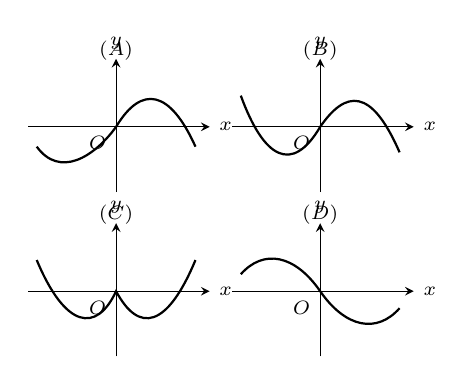
\begin{tikzpicture}[>=stealth, scale=0.72]
  \begin{scope}
    \node[font=\scriptsize] at (0,1.35) {$(A)$};
    \draw[->] (-1.55,0)--(1.65,0) node[right, font=\scriptsize] {$x$};
    \draw[->] (0,-1.15)--(0,1.2) node[above, font=\scriptsize] {$y$};
    \draw[thick] (-1.4,-0.35) .. controls (-1.0,-0.9) and (-0.4,-0.55) .. (0,0)
      .. controls (0.45,0.75) and (0.95,0.65) .. (1.4,-0.35);
    \node[below left, font=\scriptsize] at (0,0) {$O$};
  \end{scope}

  \begin{scope}[xshift=3.6cm]
    \node[font=\scriptsize] at (0,1.35) {$(B)$};
    \draw[->] (-1.55,0)--(1.65,0) node[right, font=\scriptsize] {$x$};
    \draw[->] (0,-1.15)--(0,1.2) node[above, font=\scriptsize] {$y$};
    \draw[thick] (-1.4,0.55) .. controls (-1.0,-0.55) and (-0.5,-0.85) .. (0,0)
      .. controls (0.45,0.65) and (0.9,0.7) .. (1.4,-0.45);
    \node[below left, font=\scriptsize] at (0,0) {$O$};
  \end{scope}

  \begin{scope}[yshift=-2.9cm]
    \node[font=\scriptsize] at (0,1.35) {$(C)$};
    \draw[->] (-1.55,0)--(1.65,0) node[right, font=\scriptsize] {$x$};
    \draw[->] (0,-1.15)--(0,1.2) node[above, font=\scriptsize] {$y$};
    \draw[thick] (-1.4,0.55) .. controls (-0.9,-0.65) and (-0.35,-0.75) .. (0,0)
      .. controls (0.4,-0.75) and (0.9,-0.65) .. (1.4,0.55);
    \node[below left, font=\scriptsize] at (0,0) {$O$};
  \end{scope}

  \begin{scope}[xshift=3.6cm,yshift=-2.9cm]
    \node[font=\scriptsize] at (0,1.35) {$(D)$};
    \draw[->] (-1.55,0)--(1.65,0) node[right, font=\scriptsize] {$x$};
    \draw[->] (0,-1.15)--(0,1.2) node[above, font=\scriptsize] {$y$};
    \draw[thick] (-1.4,0.3) .. controls (-1.0,0.75) and (-0.45,0.65) .. (0,0)
      .. controls (0.45,-0.65) and (1.0,-0.75) .. (1.4,-0.3);
    \node[below left, font=\scriptsize] at (0,0) {$O$};
  \end{scope}
\end{tikzpicture}
\end{center}
\nopagebreak[4]
\Needspace{4\baselineskip}
\textbf{解析}

$f(x)=-x\cos x$ 是奇函数，$f(0)=0$ 且 $f'(0)=-1$，故图像关于原点对称并在原点处由左上向右下穿过。与固定源四个选项图比较，符合的是 D。

\gkanswer{答案：D}

\end{answer}
\begin{answer}
\gksolhead{6}{}

\textbf{题目}：

《中华人民共和国个人所得税法》规定，公民全月工资、薪金所得不超过 800 元的部分不必纳税，超过 800 元的部分为全月应纳税所得额，此项税款按下表分段累进计算：

\begin{center}
\begin{tabular}{lr}
\toprule
全月应纳税所得额 & 税率 \\
\midrule
不超过 500 元的部分 & 5\% \\
超过 500 元至 2000 元的部分 & 10\% \\
超过 2000 元至 5000 元的部分 & 15\% \\
…… & …… \\
\bottomrule
\end{tabular}
\end{center}

某人一月份交纳此项税款 26.78 元，则他的当月工资、薪金所得介于\mbox{（　　）}。

（A）800–900 元　　（B）900–1200 元　　（C）1200–1500 元　　（D）1500–2800 元

\Needspace{4\baselineskip}
\textbf{解析}

先对超过 800 元的应纳税所得额 $u$ 计税。前 500 元税款为 25 元，剩余 $26.78-25=1.78$ 元按 10\% 计算，对应 $17.8$ 元所得额，所以 $u=517.8$ 元，工资薪金为 $800+517.8=1317.8$ 元，落在 1200–1500 元，选 C。

\gkanswer{答案：C，1200–1500 元}

\end{answer}
\begin{answer}
\gksolhead{7}{}

\textbf{题目}：

若 $a>b>1$，$P=\sqrt{\lg a\cdot\lg b}$，$Q=\dfrac{1}{2}(\lg a+\lg b)$，$R=\lg\left(\dfrac{a+b}{2}\right)$，则\mbox{（　　）}。

（A）$R<P<Q$　　（B）$P<Q<R$　　（C）$Q<P<R$　　（D）$P<R<Q$

\Needspace{4\baselineskip}
\textbf{解析}

令 $x=\lg a$、$y=\lg b$，则 $x>y>0$。几何平均数小于算术平均数，故 $P=\sqrt{xy}<Q=(x+y)/2$。由 $\frac{a+b}{2}>\sqrt{ab}$ 且 $\lg$ 递增，得 $R>\lg\sqrt{ab}=(x+y)/2=Q$。所以 $P<Q<R$，选 B。

\gkanswer{答案：B，$P<Q<R$}

\end{answer}
\begin{answer}
\gksolhead{8}{}

\textbf{题目}：

以极坐标系中的点 $(1,1)$ 为圆心、1 为半径的圆的方程是\mbox{（　　）}。

（A）$\rho=2\cos\left(\theta-\dfrac{\pi}{4}\right)$　　（B）$\rho=2\sin\left(\theta-\dfrac{\pi}{4}\right)$

（C）$\rho=2\cos(\theta-1)$　　（D）$\rho=2\sin(\theta-1)$

\Needspace{4\baselineskip}
\textbf{解析}

圆心极坐标为 $(1,1)$，半径为1。圆经过极点，极坐标方程为 $\rho=2\cos(\theta-1)$，选 C。

\gkanswer{答案：C}

\end{answer}
\begin{answer}
\gksolhead{9}{}

\textbf{题目}：

一个圆柱的侧面展开图是一个正方形，这个圆柱的全面积与侧面积的比是\mbox{（　　）}。

（A）$\dfrac{1+2\pi}{2\pi}$　　（B）$\dfrac{1+4\pi}{4\pi}$　　（C）$\dfrac{1+2\pi}{\pi}$　　（D）$\dfrac{1+4\pi}{2\pi}$

\Needspace{4\baselineskip}
\textbf{解析}

\Needspace{5\baselineskip}
侧面展开为正方形，所以圆柱高 $h=2\pi r$。侧面积为 $2\pi r h=4\pi^2r^2$，全面积与侧面积之比为
\nopagebreak[4]
\[
\frac{4\pi^2r^2+2\pi r^2}{4\pi^2r^2}=\frac{1+2\pi}{2\pi},
\]
选 A。

\gkanswer{答案：A，$\frac{1+2\pi}{2\pi}$}

\end{answer}
\begin{answer}
\gksolhead{10}{}

\textbf{题目}：

过原点的直线与圆 $x^2+y^2+4x+3=0$ 相切，若切点在第三象限，则该直线的方程是\mbox{（　　）}。

（A）$y=\sqrt{3}x$　　（B）$y=-\sqrt{3}x$　　（C）$y=\dfrac{\sqrt{3}}{3}x$　　（D）$y=-\dfrac{\sqrt{3}}{3}x$

\Needspace{4\baselineskip}
\textbf{解析}

圆心为 $(-2,0)$、半径为1。设过原点的切线斜率为 $m$，圆心到直线 $y=mx$ 的距离等于1，故 $2|m|/\sqrt{1+m^2}=1$，得 $m=\pm1/\sqrt3$。第三象限切点对应正斜率，选 C。

\gkanswer{答案：C，$y=\frac{\sqrt3}{3}x$}

\end{answer}
\begin{answer}
\gksolhead{11}{}

\textbf{题目}：

过抛物线 $y=ax^2\ (a>0)$ 的焦点 $F$ 作一直线交抛物线于 $P,Q$ 两点，若线段 $PF$ 与 $FQ$ 的长分别是 $p,q$，则 $\dfrac{1}{p}+\dfrac{1}{q}$ 等于\mbox{（　　）}。

（A）$2a$　　（B）$\dfrac{1}{2a}$　　（C）$4a$　　（D）$\dfrac{4}{a}$

\Needspace{4\baselineskip}
\textbf{解析}

\Needspace{5\baselineskip}
将抛物线写为 $x^2=4p_fy$，其中 $p_f=1/(4a)$。焦点弦两端点的参数 $t,s$ 满足 $ts=-1$，它们到焦点的距离分别为 $p_f(1+t^2)$ 与 $p_f(1+s^2)$。于是
\nopagebreak[4]
\[
\frac1{PF}+\frac1{FQ}
=\frac1{p_f(1+t^2)}+\frac1{p_f(1+s^2)}
=\frac1{p_f}=4a,
\]
选 C。

\gkanswer{答案：C，$4a$}

\end{answer}
\begin{answer}
\gksolhead{12}{}

\textbf{题目}：

如图，$OA$ 是圆锥底面中心 $O$ 到母线的垂线，$OA$ 绕轴旋转一周所得曲面将圆锥分成体积相等的两部分，则母线与轴的夹角的余弦值为\mbox{（　　）}。
\nopagebreak[4]
\begin{center}% 2000 年广东卷第 12 题：圆锥轴截面与 OA
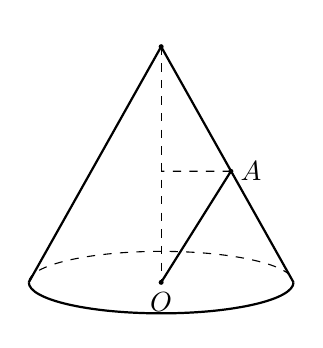
\begin{tikzpicture}[>=stealth, scale=0.82]
  \coordinate (V) at (0,3.65);
  \coordinate (O) at (0,0);
  \coordinate (L) at (-2.05,0);
  \coordinate (R) at (2.05,0);
  \coordinate (A) at (1.08,1.72);
  \draw[thick] (V)--(L) (V)--(R);
  \draw[thick] (L) arc (180:360:2.05 and 0.48);
  \draw[dashed] (L) arc (180:0:2.05 and 0.48);
  \draw[dashed] (V)--(O);
  \draw[thick] (O)--(A);
  \draw[dashed] (A)--(0,1.72);
  \fill (V) circle (1.1pt);
  \fill (O) circle (1.1pt) node[below] {$O$};
  \fill (A) circle (1.1pt) node[right] {$A$};
  \node[above] at (V) { };
\end{tikzpicture}
\end{center}
\nopagebreak[4]
（A）$\dfrac{1}{\sqrt[3]{2}}$　　（B）$\dfrac{1}{2}$　　（C）$\dfrac{1}{\sqrt{2}}$　　（D）$\dfrac{1}{\sqrt[4]{2}}$

\Needspace{4\baselineskip}
\textbf{解析}

\textbf{待核。}

\Needspace{5\baselineskip}
按题面字面，设圆锥高为 $h$、底半径为 $r$，母线与轴夹角为 $\theta$。在轴截面中令 $O=(0,0)$、顶点 $V=(0,h)$、底边缘点 $B=(r,0)$，母线 $VB$ 方程为 $hx+rz=hr$。从 $O$ 向 $VB$ 作垂线，垂足坐标为
\nopagebreak[4]
\[
A=\left(\frac{rh^2}{h^2+r^2},\frac{hr^2}{h^2+r^2}\right)
=(r\cos^2\theta,h\sin^2\theta).
\]
$OA$ 绕轴形成的内侧圆锥与原圆锥体积之比为 $\cos^4\theta\sin^2\theta$。令 $u=\cos^2\theta$，其最大值为 $u^2(1-u)|_{u=2/3}=4/27<1/2$，因此不可能满足“分成体积相等的两部分”。固定扫描件的高分辨率复核仍为该文字和图示；需查找同版勘误或独立版本，不能按选项猜填答案。

\gkanswer{答案：U/PENDING}

\end{answer}
\gkpart{二、填空题}

\begin{answer}
\gksolhead{13}{}

\textbf{题目}：

乒乓球队的 10 名队员中有 3 名主力队员，派 5 名参加比赛，3 名主力队员要安排在第一、三、五位置，其余 7 名队员选 2 名安排在第二、四位置，那么不同的出场安排共有 \gkblank{} 种（用数字作答）。

\Needspace{4\baselineskip}
\textbf{解析}

三名主力分别排入第1、3、5位，有 $3!$ 种排法。其余两位从7人中有序选取，有 $7\cdot6$ 种。总数为 $3!\cdot7\cdot6=252$。

\gkanswer{答案：$252$}

\end{answer}
\begin{answer}
\gksolhead{14}{}

\textbf{题目}：

椭圆 $\dfrac{x^2}{9}+\dfrac{y^2}{4}=1$ 的焦点为 $F_1,F_2$，$P$ 为其上的动点，当 $\angle F_1PF_2$ 为钝角时，点 $P$ 横坐标的取值范围是 \gkblank{}。

\Needspace{4\baselineskip}
\textbf{解析}

\Needspace{5\baselineskip}
椭圆焦点为 $F_1=(-\sqrt5,0)$、$F_2=(\sqrt5,0)$。钝角条件等价于
\nopagebreak[4]
\[
\overrightarrow{PF_1}\cdot\overrightarrow{PF_2}=x^2+y^2-5<0.
\]
椭圆上 $y^2=4-4x^2/9$，所以 $x^2+y^2=4+5x^2/9$。解得 $x^2<9/5$，即 $-3/\sqrt5<x<3/\sqrt5$；等号处夹角为直角，端点不取。

\gkanswer{答案：$(-3/\sqrt5,3/\sqrt5)$}

\end{answer}
\begin{answer}
\gksolhead{15}{}

\textbf{题目}：

\Needspace{5\baselineskip}
设 $\{a_n\}$ 是首项为 1 的正项数列，且
\nopagebreak[4]
\[
(n+1)a_{n+1}^{2}-na_n^{2}+a_{n+1}a_n=0\qquad(n=1,2,3,\ldots),
\]
则它的通项公式是 $a_n=$ \gkblank{}。

\Needspace{4\baselineskip}
\textbf{解析}

\Needspace{5\baselineskip}
因 $a_n>0$，令 $r_n=a_{n+1}/a_n>0$。递推式除以 $a_n^2$ 得
\nopagebreak[4]
\[
(n+1)r_n^2+r_n-n=0.
\]
正根为 $r_n=n/(n+1)$。结合 $a_1=1$，逐项相乘得 $a_n=1/n$。

\gkanswer{答案：$a_n=1/n$}

\end{answer}
\begin{answer}
\gksolhead{16}{}

\textbf{题目}：

如图，$E,F$ 分别为正方体面 $ADD_1A_1$、面 $BCC_1B_1$ 的中心，则四边形 $BFD_1E$ 在该正方体的面上的射影可能是 \gkblank{}。（要求：把可能的图序号都填上。）
\nopagebreak[4]
\begin{center}% 2000 年广东卷第 16 题：正方体内四边形投影的可能图形
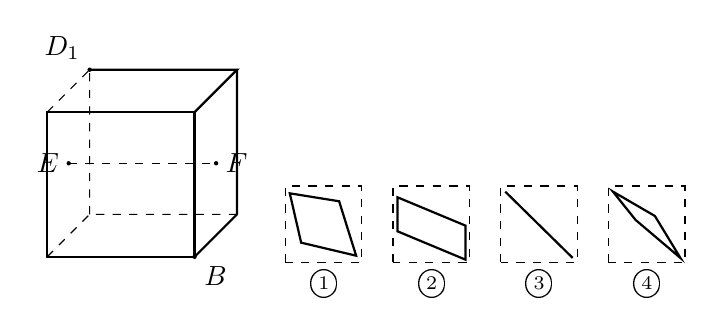
\begin{tikzpicture}[>=stealth, scale=0.72]
  \coordinate (A) at (0,0);
  \coordinate (B) at (2.6,0);
  \coordinate (C) at (3.35,0.75);
  \coordinate (D) at (0.75,0.75);
  \coordinate (A1) at (0,2.55);
  \coordinate (B1) at (2.6,2.55);
  \coordinate (C1) at (3.35,3.3);
  \coordinate (D1) at (0.75,3.3);
  \coordinate (E) at (0.38,1.65);
  \coordinate (F) at (2.98,1.65);

  \draw[thick] (A)--(B)--(B1)--(A1)--cycle;
  \draw[thick] (B1)--(C1)--(D1);
  \draw[dashed] (A)--(D)--(C) (D)--(D1) (A1)--(D1);
  \draw[thick] (B)--(C) (C)--(C1);
  \draw[dashed] (E)--(F);
  \fill (B) circle (1.1pt) node[below right] {$B$};
  \fill (D1) circle (1.1pt) node[above left] {$D_1$};
  \fill (E) circle (1.1pt) node[left] {$E$};
  \fill (F) circle (1.1pt) node[right] {$F$};

  \begin{scope}[xshift=4.2cm,yshift=-0.1cm]
    \draw[dashed] (0,0) rectangle (1.35,1.35);
    \draw[thick] (0.08,1.22)--(0.95,1.08)--(1.25,0.12)--(0.28,0.35)--cycle;
    \node[below] at (0.68,-0.08) {\textcircled{\scriptsize 1}};
  \end{scope}
  \begin{scope}[xshift=6.1cm,yshift=-0.1cm]
    \draw[dashed] (0,0) rectangle (1.35,1.35);
    \draw[thick] (0.08,1.15)--(0.08,0.55)--(1.28,0.05)--(1.28,0.65)--cycle;
    \node[below] at (0.68,-0.08) {\textcircled{\scriptsize 2}};
  \end{scope}
  \begin{scope}[xshift=8.0cm,yshift=-0.1cm]
    \draw[dashed] (0,0) rectangle (1.35,1.35);
    \draw[thick] (0.08,1.25)--(1.27,0.08);
    \node[below] at (0.68,-0.08) {\textcircled{\scriptsize 3}};
  \end{scope}
  \begin{scope}[xshift=9.9cm,yshift=-0.1cm]
    \draw[dashed] (0,0) rectangle (1.35,1.35);
    \draw[thick] (0.08,1.25)--(0.48,0.75)--(1.27,0.08)--(0.82,0.82)--cycle;
    \node[below] at (0.68,-0.08) {\textcircled{\scriptsize 4}};
  \end{scope}
\end{tikzpicture}
\end{center}
\nopagebreak[4]
\Needspace{4\baselineskip}
\textbf{解析}

设正方体顶点坐标为 $A=(0,0,0)$、$B=(1,0,0)$、$C=(1,1,0)$、$D=(0,1,0)$，上底各点的第三坐标为1。则 $E=(0,1/2,1/2)$、$F=(1,1/2,1/2)$、$D_1=(0,1,1)$。投影到 $x=0$ 面时，四个顶点依次投到 $A,E,D_1,E$，落在对角线 $AD_1$ 上；投影到 $x=1$ 面时依次投到 $B,F,C_1,F$，落在对角线 $BC_1$ 上，均对应选项③。投影到 $y=0,1$ 或 $z=0,1$ 面时，四个投影点构成选项②所示的平行四边形。因此可能图形为②、③。

\gkanswer{答案：②、③}

\end{answer}
\gkpart{三、解答题}

\begin{answer}
\gksolhead{17}{}

\textbf{题目}：

已知函数 $y=\sqrt{3}\sin x+\cos x$，$x\in\mathbb{R}$。

（1） 当函数 $y$ 取得最大值时，求自变量 $x$ 的集合；

（2） 该函数的图象可由 $y=\sin x\ (x\in\mathbb{R})$ 的图象经过怎样的平移和伸缩变换得到？

\Needspace{4\baselineskip}
\textbf{解析}

\nopagebreak[4]
\[
y=\sqrt3\sin x+\cos x=2\sin\left(x+\frac\pi6\right).
\]
\gksubpart{（1）}

最大值在 $x+\pi/6=\pi/2+2k\pi$ 时取得，故 $x=\pi/3+2k\pi$，$k\in\mathbb Z$。

\gksubpart{（2）}

先将 $y=\sin x$ 的图像向左平移 $\pi/6$，再沿纵轴方向伸长为原来的2倍。

\gkanswer{答案（1）：$x=\pi/3+2k\pi$，$k\in\mathbb Z$}

\gkanswer{答案（2）：先左移 $\pi/6$，再沿纵轴伸长为原来的2倍}

\end{answer}
\begin{answer}
\gksolhead{18}{}

\textbf{题目}：

\Needspace{5\baselineskip}
设 $\{a_n\}$ 为等比数列，
\nopagebreak[4]
\[
T_n=na_1+(n-1)a_2+\cdots+2a_{n-1}+a_n,
\]
已知 $T_1=1,\ T_2=4$。

（1） 求数列 $\{a_n\}$ 的首项和公比；

（2） 求数列 $\{T_n\}$ 的通项公式。

\Needspace{4\baselineskip}
\textbf{解析}

\gksubpart{（1）}

$T_1=a_1=1$，且 $T_2=2a_1+a_2=4$，所以 $a_1=1$、$a_2=2$，公比 $q=2$。

\gksubpart{（2）}

\Needspace{5\baselineskip}
于是
\nopagebreak[4]
\[
T_n=\sum_{k=1}^n(n-k+1)2^{k-1}=2^{n+1}-n-2.
\]
代入 $n=1,2$ 可分别得到 $T_1=1$、$T_2=4$。

\gkanswer{答案（1）：$a_1=1$，公比 $q=2$}

\gkanswer{答案（2）：$T_n=2^{n+1}-n-2$}

\end{answer}
\begin{answer}
\gksolhead{19}{}

\textbf{题目}：

如图，已知平行六面体 $ABCD-A_1B_1C_1D_1$ 的底面 $ABCD$ 上菱形，且 $\angle C_1CB=\angle C_1CD=\angle BCD$。

\begin{gktip}
\textbf{源文待核（ISSUE-1201）}：固定扫描件照录为“底面 $ABCD$ 上菱形”；此处语义不通，暂不擅自补字或改写。
\end{gktip}

（1） 证明：$C_1C\perp BD$；

（2） 当 $\dfrac{CD}{CC_1}$ 的值为多少时，能使 $A_1C\perp$ 平面 $C_1BD$？请给出证明。
\nopagebreak[4]
\begin{center}% 2000 年广东卷第 19 题：平行六面体 ABCD-A1B1C1D1
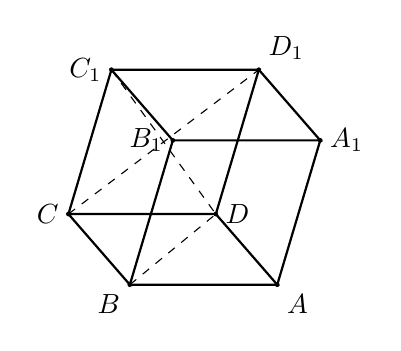
\begin{tikzpicture}[>=stealth, scale=0.78]
  \coordinate (A) at (3.4,0);
  \coordinate (B) at (1.0,0);
  \coordinate (C) at (0,1.15);
  \coordinate (D) at (2.4,1.15);
  \coordinate (A1) at (4.1,2.35);
  \coordinate (B1) at (1.7,2.35);
  \coordinate (C1) at (0.7,3.5);
  \coordinate (D1) at (3.1,3.5);

  \draw[thick] (A)--(B)--(C)--(D)--cycle;
  \draw[thick] (A1)--(B1)--(C1)--(D1)--cycle;
  \draw[thick] (A)--(A1) (B)--(B1) (C)--(C1) (D)--(D1);
  \draw[dashed] (C1)--(D) (B)--(D) (C)--(D1);

  \fill (A) circle (1.1pt) node[below right] {$A$};
  \fill (B) circle (1.1pt) node[below left] {$B$};
  \fill (C) circle (1.1pt) node[left] {$C$};
  \fill (D) circle (1.1pt) node[right] {$D$};
  \fill (A1) circle (1.1pt) node[right] {$A_1$};
  \fill (B1) circle (1.1pt) node[left] {$B_1$};
  \fill (C1) circle (1.1pt) node[left] {$C_1$};
  \fill (D1) circle (1.1pt) node[above right] {$D_1$};
\end{tikzpicture}
\end{center}
\nopagebreak[4]
\Needspace{4\baselineskip}
\textbf{解析}

固定扫描原字为“底面 $ABCD$ 上菱形”，本题源文语义待核（ISSUE-1201、ISSUE-1202）。以下两问仅在假设“上”本意为“是”、即 $ABCD$ 为菱形时成立；此释读未获来源确认。

\gksubpart{（1）}

\Needspace{5\baselineskip}
令 $C$ 为原点，记 $\mathbf u=\overrightarrow{CB}$、$\mathbf v=\overrightarrow{CD}$、$\mathbf w=\overrightarrow{CC_1}$，且 $|\mathbf u|=|\mathbf v|=s$、$|\mathbf w|=L$、$\angle BCD=\theta$。由题设两个夹角相等，$\mathbf w\cdot\mathbf u=\mathbf w\cdot\mathbf v$，故
\nopagebreak[4]
\[
\mathbf w\cdot\overrightarrow{BD}=\mathbf w\cdot(\mathbf v-\mathbf u)=0,
\]
即 $C_1C\perp BD$。

\gksubpart{（2）}

\Needspace{5\baselineskip}
又 $\overrightarrow{CA_1}=\mathbf u+\mathbf v+\mathbf w$。它已经垂直于 $BD$；要使它垂直于平面 $C_1BD$，还须垂直于平面内的向量 $\mathbf w-\mathbf u$。计算得
\nopagebreak[4]
\[
(\mathbf u+\mathbf v+\mathbf w)\cdot(\mathbf w-\mathbf u)
=(L-s)\bigl(L+s(1+\cos\theta)\bigr).
\]
第二因子为正，故需 $L=s$，即 $CD/CC_1=1$。

\gkanswer{答案（1）：U/PENDING}

\gkanswer{答案（2）：U/PENDING}

\end{answer}
\begin{answer}
\gksolhead{20}{}

\textbf{题目}：

设函数 $f(x)=\sqrt{x^2+1}-ax$，其中 $a>0$。

（1） 解不等式 $f(x)\leq 1$；

（2） 证明：当 $a\geq1$ 时，函数 $f(x)$ 在区间 $[0,+\infty)$ 上是单调函数。

\Needspace{4\baselineskip}
\textbf{解析}

\gksubpart{（1）}

\Needspace{5\baselineskip}
不等式为 $\sqrt{x^2+1}-1\le ax$。左端非负，故 $x<0$ 无解，$x=0$ 成立。对 $x>0$，有
\nopagebreak[4]
\[
\frac{\sqrt{x^2+1}-1}{x}=\frac{x}{\sqrt{x^2+1}+1}\le a.
\]
\Needspace{5\baselineskip}
左式随 $x$ 递增。当 $0<a<1$ 时，等号点为 $x=2a/(1-a^2)$；当 $a\ge1$ 时，不等式对所有 $x\ge0$ 成立。故解集为
\nopagebreak[4]
\[
\begin{cases}[0,\frac{2a}{1-a^2}],&0<a<1,\\[3pt][0,+\infty),&a\ge1.\end{cases}
\]

\gksubpart{（2）}

\Needspace{5\baselineskip}
对 $x\ge0$，
\nopagebreak[4]
\[
f'(x)=\frac{x}{\sqrt{x^2+1}}-a<1-a\le0,
\]
所以 $f$ 在 $[0,+\infty)$ 上严格递减。

\gkanswer{答案（1）：$0<a<1$ 时 $[0,2a/(1-a^2)]$；$a\ge1$ 时 $[0,+\infty)$}

\gkanswer{答案（2）：$f$ 在 $[0,+\infty)$ 上严格递减}

\end{answer}
\begin{answer}
\gksolhead{21}{}

\textbf{题目}：

某蔬菜基地种植西红柿，由历年市场行情得知，从二月一日起的 300 天内，西红柿市场售价与上市时间的关系用图一的一条折线表示；西红柿的种植成本与上市时间的关系用图二的抛物线段表示。

（1） 写出图一表示的市场售价与时间的函数关系式 $p=f(t)$ 和图二表示的种植成本与时间的函数关系式 $Q=g(t)$；

（2） 认定市场售价减去种植成本为纯收益，问何时上市的西红柿纯收益最大？

注：市场售价各种植成本的单位：元/$10^2\,\mathrm{kg}$，时间单位：天。
\nopagebreak[4]
\begin{center}% 2000 年广东卷第 21 题：市场售价与种植成本图象
\begin{tikzpicture}[>=stealth, scale=0.78]
  \begin{scope}
    \draw[->] (0,0)--(3.55,0) node[right] {$t$};
    \draw[->] (0,0)--(0,3.65) node[above] {$P$};
    \draw[thick] (0,3.0)--(2.0,1.0)--(3.0,3.0);
    \draw[dashed] (0,3.0)--(3.0,3.0) (0,1.0)--(2.0,1.0)
      (2.0,0)--(2.0,1.0) (3.0,0)--(3.0,3.0);
    \node[left, font=\scriptsize] at (0,3.0) {300};
    \node[left, font=\scriptsize] at (0,1.0) {100};
    \node[below, font=\scriptsize] at (2.0,0) {200};
    \node[below, font=\scriptsize] at (3.0,0) {300};
    \node[below] at (1.5,-0.42) {图一};
  \end{scope}
  \begin{scope}[xshift=4.35cm]
    \draw[->] (0,0)--(3.55,0) node[right] {$t$};
    \draw[->] (0,0)--(0,3.65) node[above] {$Q$};
    \draw[thick, domain=0:3, samples=80]
      plot (\x,{1+(\x-1.5)^2/2});
    \draw[dashed] (0,1)--(3,1) (0,1.5)--(0.5,1.5) (0,1.5)--(2.5,1.5)
      (0.5,0)--(0.5,1.5) (1.5,0)--(1.5,1) (2.5,0)--(2.5,1.5);
    \node[left, font=\scriptsize] at (0,3.0) {300};
    \node[left, font=\scriptsize] at (0,2.5) {250};
    \node[left, font=\scriptsize] at (0,1.5) {150};
    \node[left, font=\scriptsize] at (0,1.0) {100};
    \node[below, font=\scriptsize] at (0.5,0) {50};
    \node[below, font=\scriptsize] at (1.5,0) {150};
    \node[below, font=\scriptsize] at (2.5,0) {250};
    \node[below] at (1.5,-0.42) {图二};
  \end{scope}
\end{tikzpicture}
\end{center}
\nopagebreak[4]
\Needspace{4\baselineskip}
\textbf{解析}

\gksubpart{（1）}

\Needspace{5\baselineskip}
从图一读出折线经过 $(0,300)$、$(200,100)$、$(300,300)$，所以
\nopagebreak[4]
\[
p(t)=\begin{cases}300-t,&0\le t\le200,\\2t-300,&200\le t\le300.\end{cases}
\]
\Needspace{5\baselineskip}
图二抛物线顶点为 $(150,100)$，并经过 $(50,150)$、$(250,150)$，故
\nopagebreak[4]
\[
Q(t)=\frac{(t-150)^2}{200}+100\qquad(0\le t\le300).
\]
\gksubpart{（2）}

\Needspace{5\baselineskip}
纯收益 $R(t)=p(t)-Q(t)$。在 $0\le t\le200$ 时，
\nopagebreak[4]
\[
R(t)=87.5+0.5t-\frac{t^2}{200},
\]
\Needspace{5\baselineskip}
其最大值在顶点 $t=50$ 处取得，值为100。在 $200\le t\le300$ 时，
\nopagebreak[4]
\[
R(t)=3.5t-512.5-\frac{t^2}{200},
\]
导数 $3.5-t/100>0$，故该段最大值在 $t=300$ 处，为87.5。全域最大收益在第50天取得。

\gkanswer{答案（1）：$p(t)=300-t$（$0\le t\le200$），$p(t)=2t-300$（$200\le t\le300$）；$Q(t)=(t-150)^2/200+100$}

\gkanswer{答案（2）：图中 $t=50$ 天时纯收益最大}

\end{answer}
\begin{answer}
\gksolhead{22}{}

\textbf{题目}：

如图，已知梯形 $ABCD$ 中 $|AB|=2|CD|$，点 $E$ 分有向线段 $AC$ 所成的比为 $\lambda$，双曲线过 $C,D,E$ 三点，且以 $A,B$ 为焦点。当 $\dfrac{2}{3}\leq\lambda\leq\dfrac{3}{4}$ 时，求双曲线离心率 $e$ 的取值范围。
\nopagebreak[4]
\begin{center}% 2000 年广东卷第 22 题：梯形、分点与双曲线
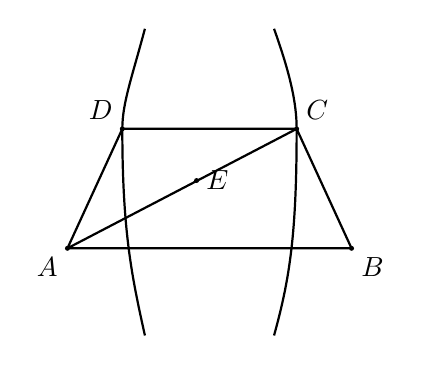
\begin{tikzpicture}[>=stealth, scale=0.82]
  \coordinate (A) at (0,0);
  \coordinate (B) at (4.4,0);
  \coordinate (D) at (0.85,1.85);
  \coordinate (C) at (3.55,1.85);
  \coordinate (E) at (2.0,1.05);

  \draw[thick] (A)--(B)--(C)--(D)--cycle;
  \draw[thick] (A)--(C);
  \draw[thick] (1.2,3.4) .. controls (1.0,2.65) and (0.85,2.25) .. (0.85,1.85);
  \draw[thick] (3.2,3.4) .. controls (3.45,2.7) and (3.55,2.25) .. (3.55,1.85);
  \draw[thick] (1.2,-1.35) .. controls (1.0,-0.45) and (0.85,0.25) .. (0.85,1.85);
  \draw[thick] (3.2,-1.35) .. controls (3.45,-0.45) and (3.55,0.25) .. (3.55,1.85);

  \fill (A) circle (1.1pt) node[below left] {$A$};
  \fill (B) circle (1.1pt) node[below right] {$B$};
  \fill (C) circle (1.1pt) node[above right] {$C$};
  \fill (D) circle (1.1pt) node[above left] {$D$};
  \fill (E) circle (1.1pt) node[right] {$E$};
\end{tikzpicture}
\end{center}
\nopagebreak[4]
\Needspace{4\baselineskip}
\textbf{解析}

\textbf{条件推导。}

固定源未说明有向分点比的分子和分母顺序；以下仅在 $\lambda=AE/EC$ 时成立，最终答案保留为 \texttt{U/PENDING}。令 $AB=2c$，以 $AB$ 为焦点轴，取 $A=(-c,0)$、$B=(c,0)$。由 $CD=c$、$CD\parallel AB$，且 $C,D$ 位于双曲线两支，可设 $C=(c/2,h)$、$D=(-c/2,h)$。设 $S=AC$、$T=BC$，则 $S^2-T^2=2c^2$。令 $d=(S-T)/c=2e$。

\Needspace{5\baselineskip}
记 $t=AE/AC=\lambda/(1+\lambda)$。因 $E$ 在 $AC$ 上且位于左支，$AE=tS$、$BE-AE=S-T=dc$。将坐标距离代入并化简得
\nopagebreak[4]
\[
d^2=\frac{4(1-2t)}{1+t},\qquad e^2=\frac{1-2t}{1+t}=\frac{1-\lambda}{1+2\lambda}.
\]
\Needspace{5\baselineskip}
该式在 $\lambda\in[2/3,3/4]$ 上递减，故
\nopagebreak[4]
\[
e\in\left[\frac1{\sqrt{10}},\frac1{\sqrt7}\right].
\]
因此，仅在 $\lambda=AE/EC$ 的约定下，条件范围为 $e\in[1/\sqrt{10},1/\sqrt7]$；在该定义获得来源确认前不作为最终答案。

\gkanswer{答案：U/PENDING}

\end{answer}
\end{document}
